\documentclass[a4paper,12pt]{article}

\usepackage[catalan]{babel}
\usepackage{fontspec}
\usepackage{fullpage}
\usepackage[a4paper, margin=2cm]{geometry} % To change the margins
\usepackage{graphicx} % Insert images
\usepackage[hidelinks]{hyperref} % Links color
\usepackage{import}
\usepackage{ragged2e}
\usepackage{wrapfig} %To Text wrap
\usepackage{listings} % Add code
\usepackage{tikz}
\usepackage{calc}
\usepackage{makeidx}

%Tikz defines
\usetikzlibrary{shapes, arrows, positioning, automata, calc}
\tikzstyle{UML} = [rectangle split, rectangle split parts=3, draw,text centered,
				   every two node part/.style={align=left, font=\scriptsize}, 
				   every three node part/.style={align=left, font=\scriptsize},
				   font=\scriptsize\bf]
\tikzstyle{cas} = [ellipse, draw, text centered, font=\scriptsize]
\tikzstyle{arrow} = [thick,-]
\begin{document}
%\title{\textsc{Ken-Ken} \\ \large 1a entrega PROP}
%\author{Marc Asenjo i Ponce de León \and
%	Arnau Canyadell i Miquel \and
%	Joan Marcè i Igual \and
%	Iñigo Moreno i Caireta \and
%	Esteve Tarragó i Sanchís}

%\date{\today}
%\maketitle

%\makeindex
\newpage

\section{Enunciat ampliat}


El nostre grup ha escollit fer el treball de PROP sobre el Ken-Ken. Segons Wikipedia, ``el Ken-Ken és un trencaclosques similar al Sudoku.
 Les regles són no repetir cap número en files o columnes i les regions marcades de formes diverses han 
 d'estar ocupades per números que formin la xifra exacta mitjançant les operacions indicades: suma, 
 resta, multiplicació o divisió. Els dígits poden repetir-se dins d'una regió, sempre que no es trobin 
 en la mateixa fila o columna.''
\href{https://ca.wikipedia.org/wiki/Kenken}{(Enllaç a la Wikipèdia)}
\\


En aquesta aplicació l'usuari podrà resoldre Ken-Kens amb l'assistència del programa o bé si ho prefereix podrà fer que la màquina el resolgui (fent que no pugui obtenir puntuació si en el futur decideix resoldre'l). Mentre l'usuari resolgui un Ken-Ken l'aplicació anirà comprovant el compliment de les regles del joc i en el cas que no se'n complís alguna es mostrarà un avís. Es permetrà a l'usuari desfer els moviments recents, així com, opcionalment, afegir anotacions que ajudin a recordar possibles valors d'una casella. S'atorgarà una puntuació al jugador en funció del temps que hagi durat la partida i també dels errors comesos durant aquesta. Es podrà guardar la partida a mig fer i reprendre-la en un altre moment.
\\


Hi haurà una base de dades de taulers de Ken-Ken creats per l'ordinador o per un usuari. Pels taulers que l'usuari creï el programa comprovarà que hi hagi una solució possible. Si no, el donarà com a \emph{no vàlid}. Opcionalment, l'aplicació tindrà eines que ajudin a l'usuari a crear el seu Ken-Ken, e.g. que ompli el tauler de nombres aleatoris que compleixin les restriccions de fila i columna, o que donada una regió amb uns nombres l'aplicació calculi les operacions i resultats possibles. Els Ken-Ken generats pel programa podran tenir uns patrons predefinits tals com la mida del tauler o la forma de les regions (hi haurà una llista on es podran escollir les que es volen i les que no). Opcionalment, també es podrà escollir nivell de dificultat del Ken-Ken tenint en compte factors com les operacions que poden utilitzar les regions o la quantitat de possibles combinacions de nombres que encaixen en cada regió individualment.
\\


Finalment, hi haurà una base de dades de jugadors, taulers i partides que servirà per guardar la informació en diferents instàncies de l'aplicació. Es podrà fer log in com a usuari (opcionalment s'enllaçarà aquest usuari amb xarxes socials). Hi haurà un rànquing de totes les partides i un altre rànquing de les partides de l'usuari ordenades per puntuació o temps de resolució. La base de dades de taulers contindrà tant els creats per la màquina com els creats pels usuaris.

\newpage
\section{Casos d'ús}
\subsection{Diagrama}

\begin{tikzpicture}[node distance=0.5cm and 1cm, auto, align=center]
\node(StartApp){
\includegraphics[width=1.3cm]{./Images/stickman}};
\node[cas, right = of StartApp, xshift=2cm](Create){Crear\\tauler};
\node[cas, above = of Create](Ranking){Veure\\rànquing};
\node[cas, above = of Ranking](Users){Administrar\\usuaris};
\node[cas, above = of Users, xshift=-1cm](KenKen){Administrar\\base de dades};
\node[cas, above right = of Create](CreateUser){Creat\\per l'usuari};
\node[cas, right = of Create](CreateMachine){Creat per\\la màquina};
\node[cas, below = of Create](Solve){Resoldre\\tauler};
\node[cas, right = of Solve](AutoSolve){Resoldre\\automàticament};
\node[cas, below right = of Solve](UserSolve){Usuari};

\foreach \x/\y in {StartApp/Create, StartApp/Ranking, StartApp/Users, 
				   StartApp/KenKen, StartApp/Solve, Create/CreateUser,
				   Create/CreateMachine, Solve/AutoSolve, Solve/UserSolve} 
{
	\draw[thick, ->] (\x) -- (\y);
};
\end{tikzpicture}
%MARCAR MILLOR LES PARTS OPCIONALS (CURSIVA O NEGRITA)
\paragraph{Veure rànquing:} 
L'usuari podrà veure una llista de les seves partides i de les millors dels altres jugadors, organitzades per puntuació o temps en resoldre, i podrà veure en quin tauler s'ha jugat cada una. Opcionalment es podran filtrar les partides per la mida del tauler i dificultat. 

\paragraph{Crear tauler/Creat per l'usuari:}
L'usuari seleccionarà una mida de tauler i crearà regions amb operació i resultat. A més, podrà emplenar les caselles amb números com a anotacions i, finalment, veure si el tauler té solució i si és única.

\paragraph{Crear tauler/Creat per la màquina:}
L'aplicació crearà un tauler a partir de paràmetres introduïts per l'usuari com la mida del tauler, la forma, mida i operació de les regions i la quantitat de cada tipus de regió.

\paragraph{Resoldre tauler/Usuari:}
L'usuari podrà resoldre els taulers amb el monitoratge de l'aplicació, que notificarà els errors trivials. Es tindrà l'opció de desfer els moviments més recents. Opcionalment, es podrà anotar la possibilitat que un nombre pugui estar en una determinada ce\lgem a i es podrà demanar ajuda a la màquina a canvi de perdre punts.

\newpage
\section{Diagrama de classes}
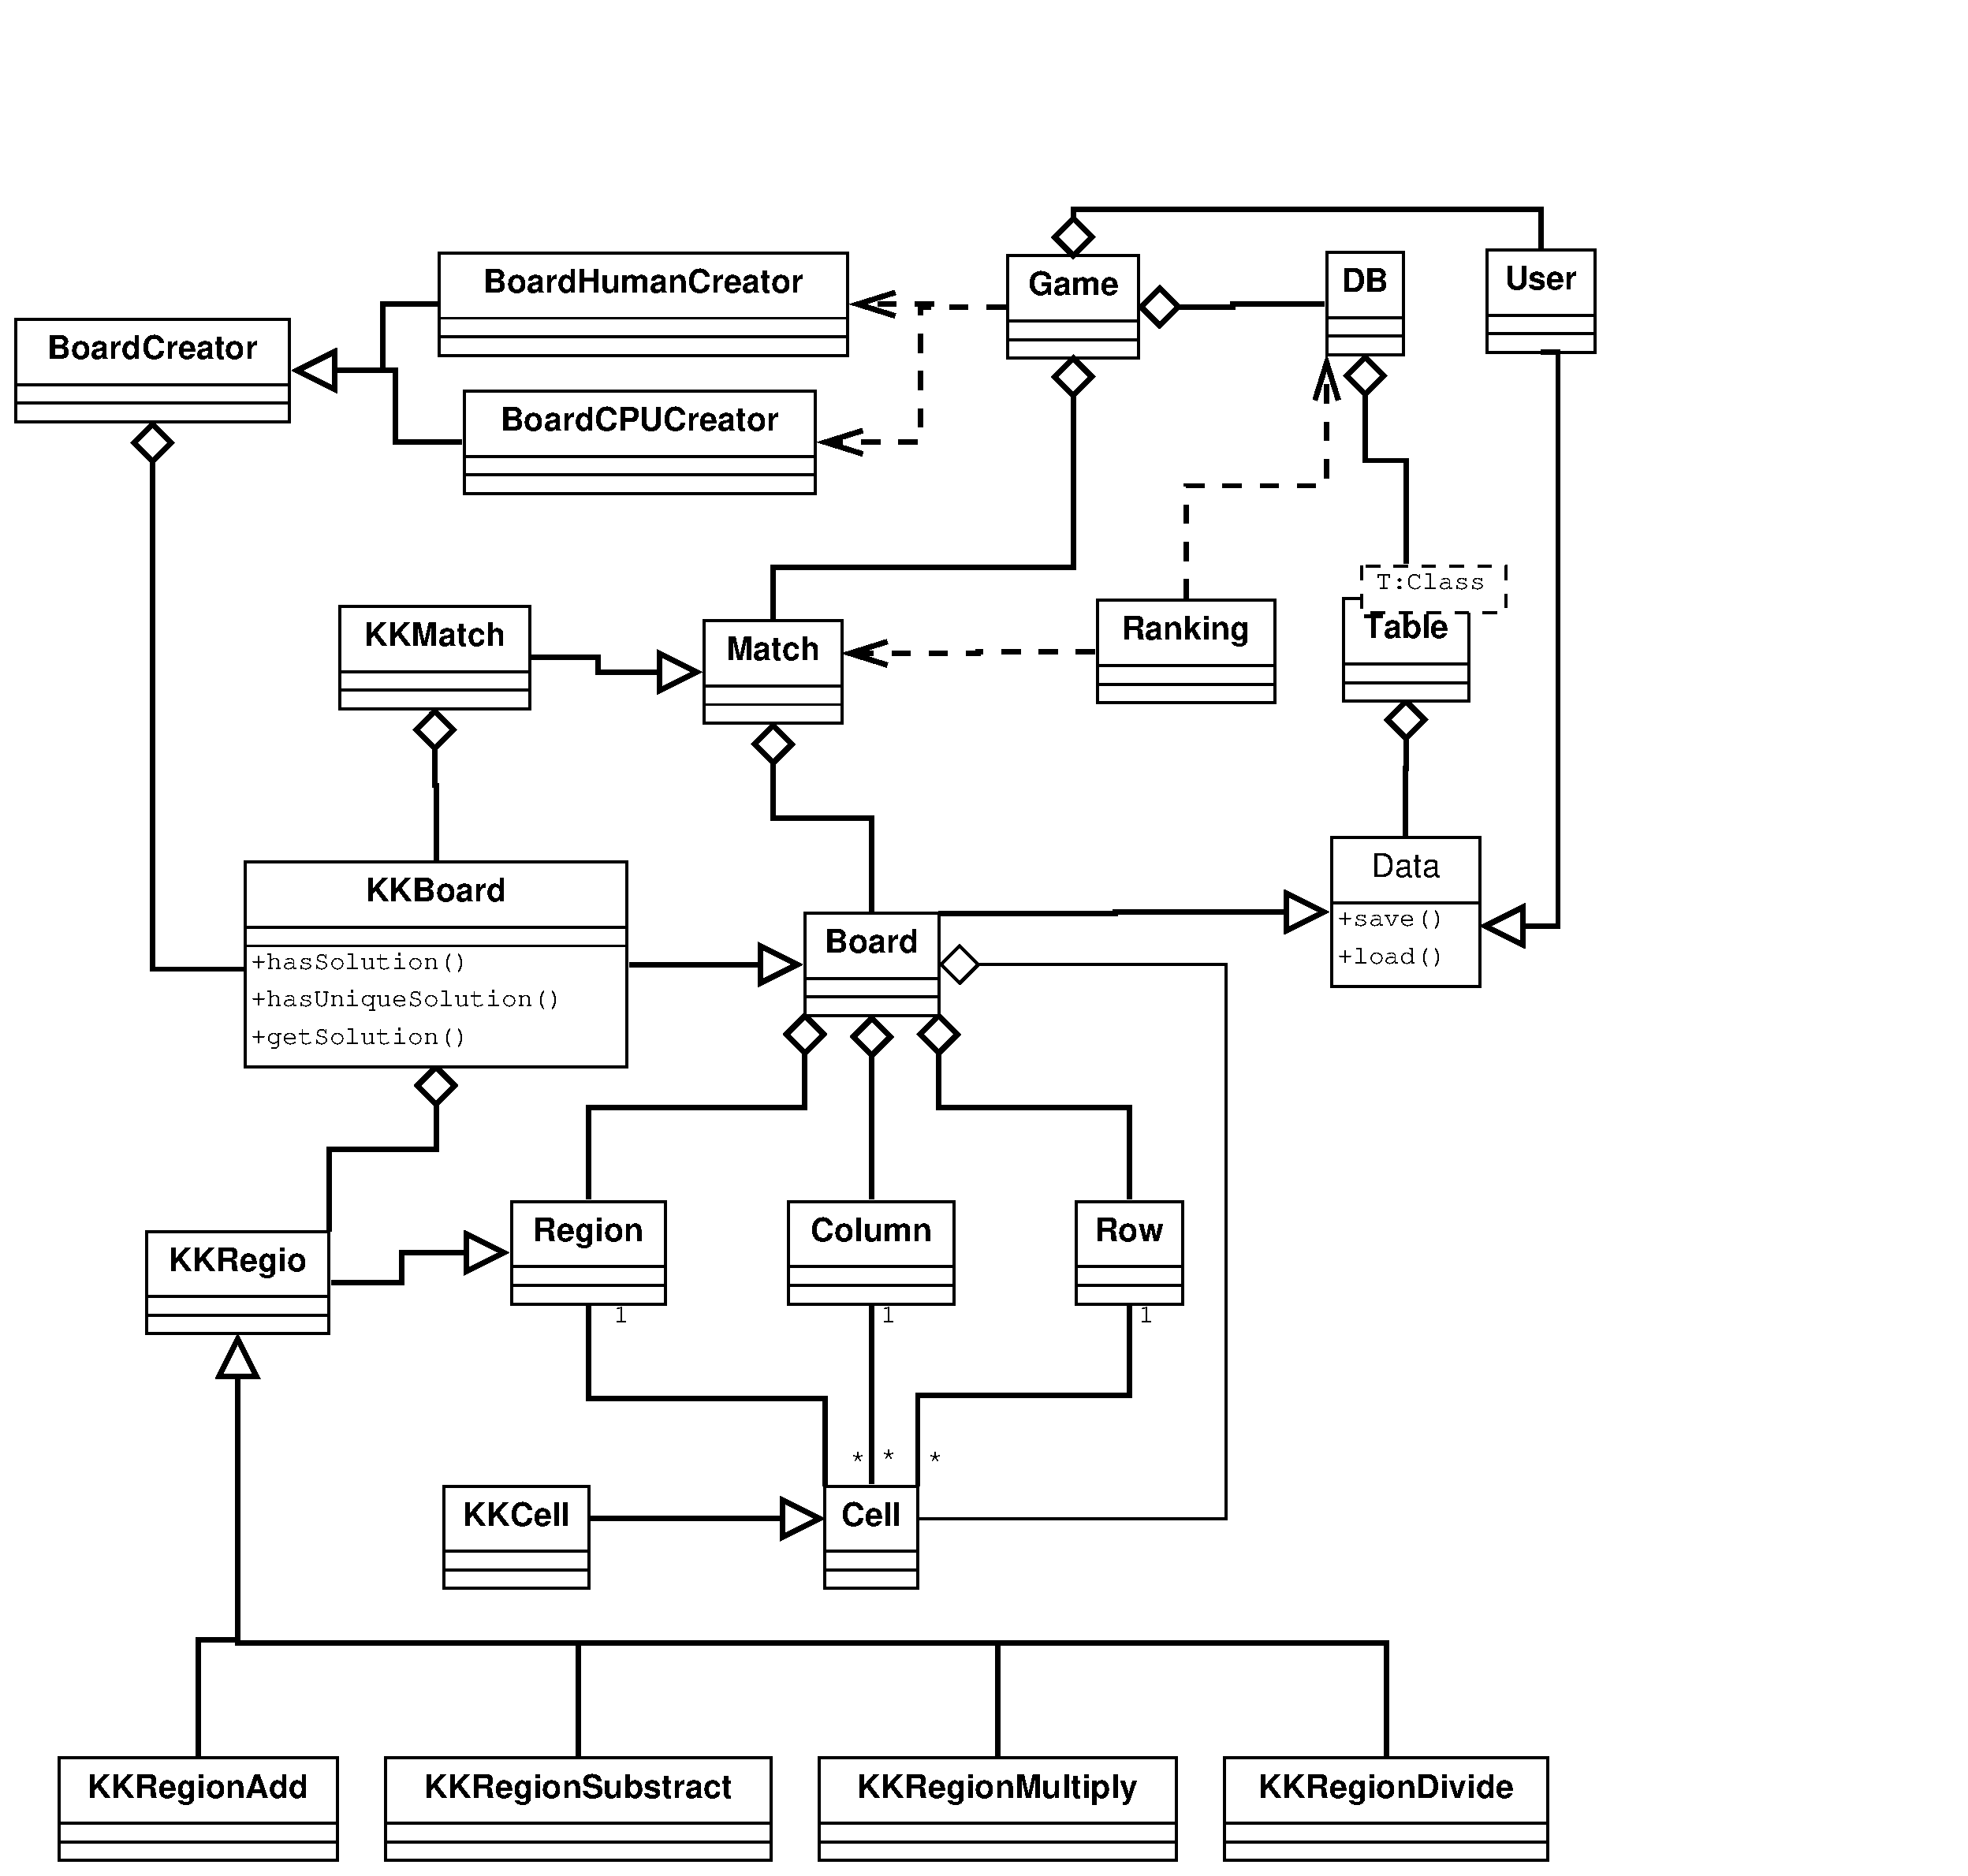
\includegraphics[width=22cm]{./Diagrama1.eps}

\newpage
\paragraph{Game:}
És la classe principal del programa que administra la BD, procedeix a l’autentificació dels usuaris, permet veure el rànquing, crear un tauler i jugar una partida.

\paragraph{DB:}És un contenidor de taules que s’encarrega de la gestió de fitxers i permet crear, carregar i guardar les taules.

\paragraph{Table:}És un contenidor de Data, que és una classe abstracta que obliga els seus fills a implementar les funcions save i load.

\paragraph{Match:}És una subclasse de Data que conté informació sobre l’estat d’una partida, que no té perquè estar acabada.

\paragraph{KKMatch:}S’encarrega de que es compleixin les restriccions durant la partida.

\paragraph{BoardCPUCreator:}És la classe encarregada de crear un tauler donades certes premisses de l’usuari.

\paragraph{BoardHumanCreator:}Permet a l’usuari construir un tauler des de zero.

\paragraph{KKBoard:}A més de ser una classe contenidora de cel·les, files, columnes i regions, conté mètodes per saber si té solució i resoldre el Ken-Ken.
\end{document}
